\documentclass{article}

\usepackage[a4paper,left=18mm,right=18mm,top=20mm,bottom=18mm]{geometry}
\usepackage[italian]{babel}

\usepackage{titling}
\usepackage{graphicx}
\usepackage{subcaption}
\usepackage{float}
\usepackage{hyperref}


\title{Grafici UML}
\author{Nicolas Anselmi, David Guzman Piedrahita and Marco Vinciguerra}
 
\begin{document}
\maketitle        
\section{Introduzione}
Nel progetto vengono fatti diversi activity diagram per illustrare al
meglio il funzionamento ai diversi tipi di stakexholder.
 
\section{Use case diagram}
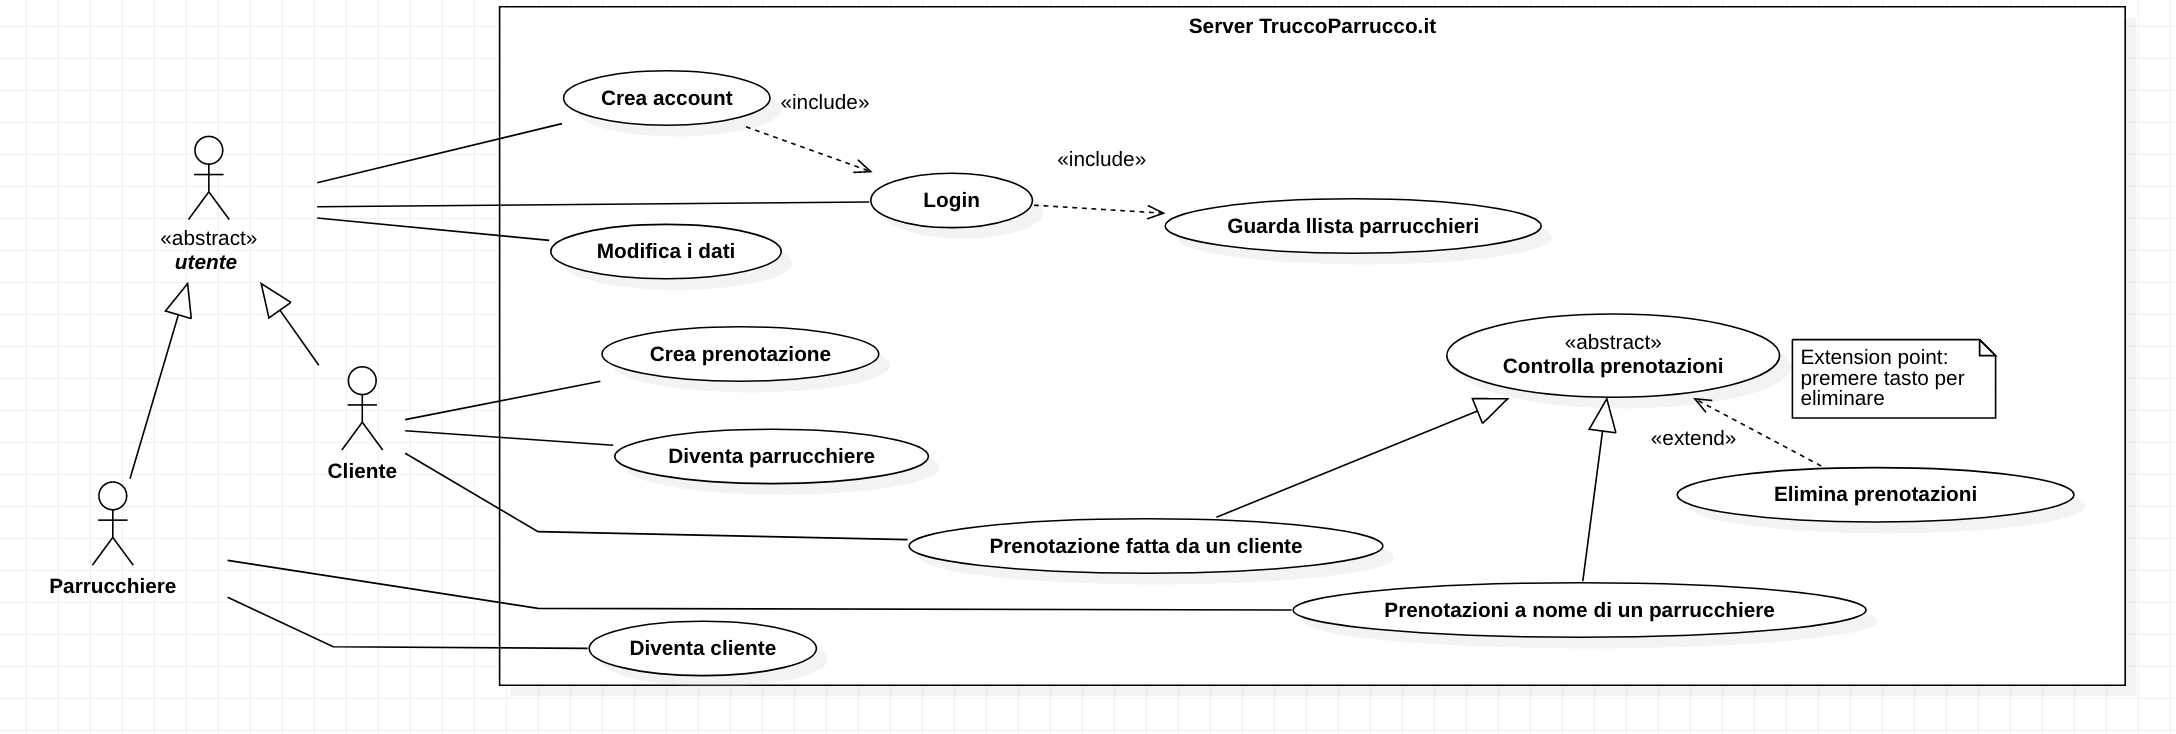
\includegraphics[scale = 0.45]{ImmaginiUML/UseCase.png}
\newpage
\section{Class diagram}
In questo le immagini a sinistra e a destra rappresentano rispettivamente l'interfaccia 
grafica fatta con Flutter e il database real time Firebase. La logica del database
non è rappresentabile con delle classi nel class diagram perchè si accede 
al servizio tramite delle API e il funzionamento non è noto.
L'interfaccia grafica invece è rappresentabile solo tramite un widget tree 
e non tramite un diagramma delle classi.
\\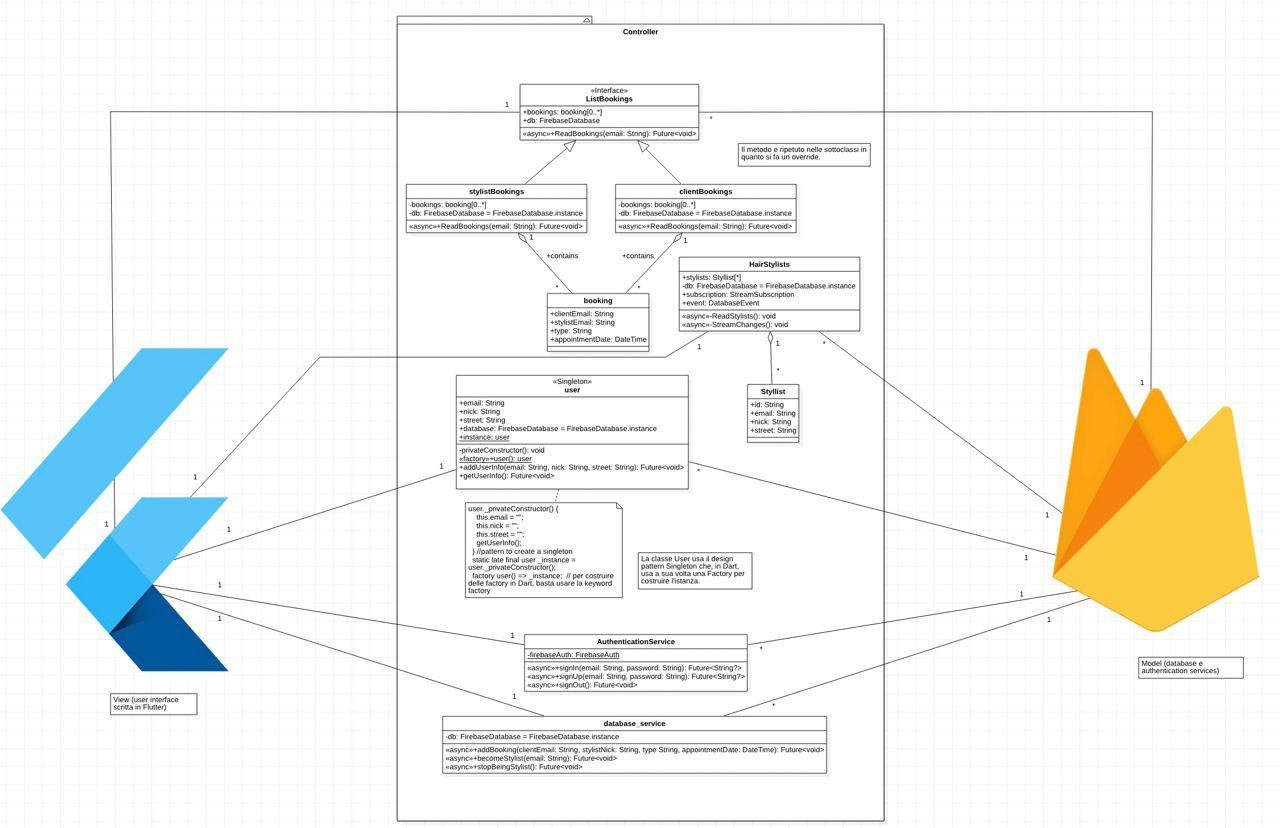
\includegraphics[scale = 0.4]{ImmaginiUML/ClassDiagram.jpg}
\newpage 
\section{State machine diagram}
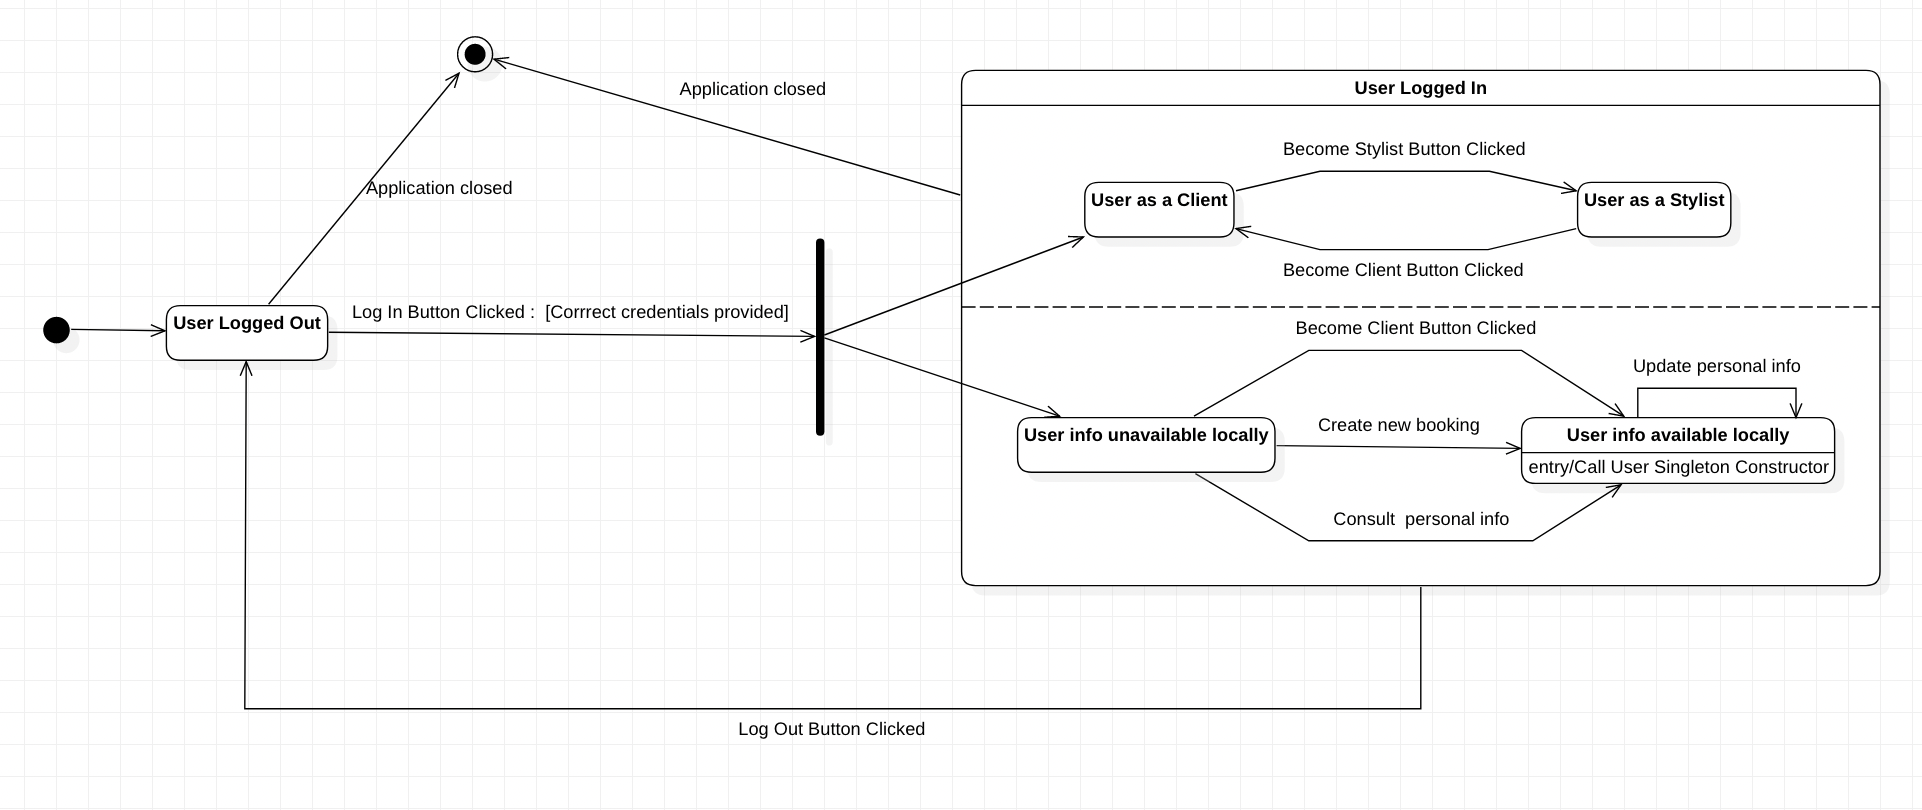
\includegraphics[scale = 0.5]{ImmaginiUML/StateMachineDiagram.png}
\newpage
\section{Sequence diagram}
\subsection{Become stylist}
\includegraphics[scale=0.45]{ImmaginiUML/Sequence1.jpg}
\subsection{Make booking}
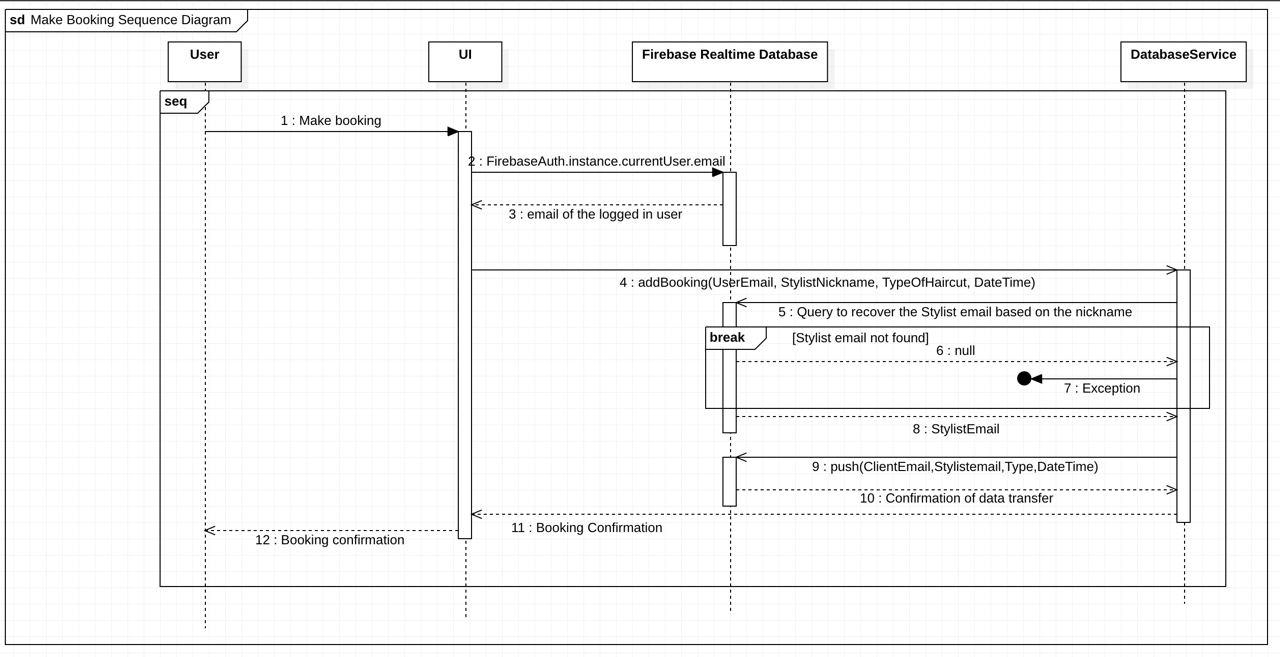
\includegraphics[scale=0.4]{ImmaginiUML/Sequence2.jpg}
\subsection{Read stylist booking}
\includegraphics[scale=0.40]{ImmaginiUML/Sequence3.jpg}

\newpage
\section{Activity diagram} 
\subsection{Spiegazione}
Sono stati fatti 3 activity diagram per rappresentare al meglio 
i divers punti di vista degli stakeholder.
\subsection{funzionamento del programma con una granularità alta}
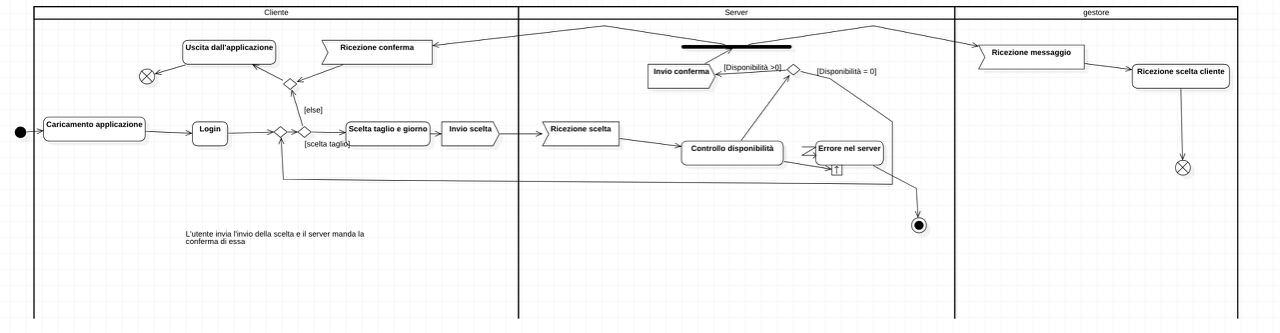
\includegraphics[scale = 0.38]{ImmaginiUML/Activity1.jpg}
\subsection{funzionamento dell'UI con i nomi delle classi}
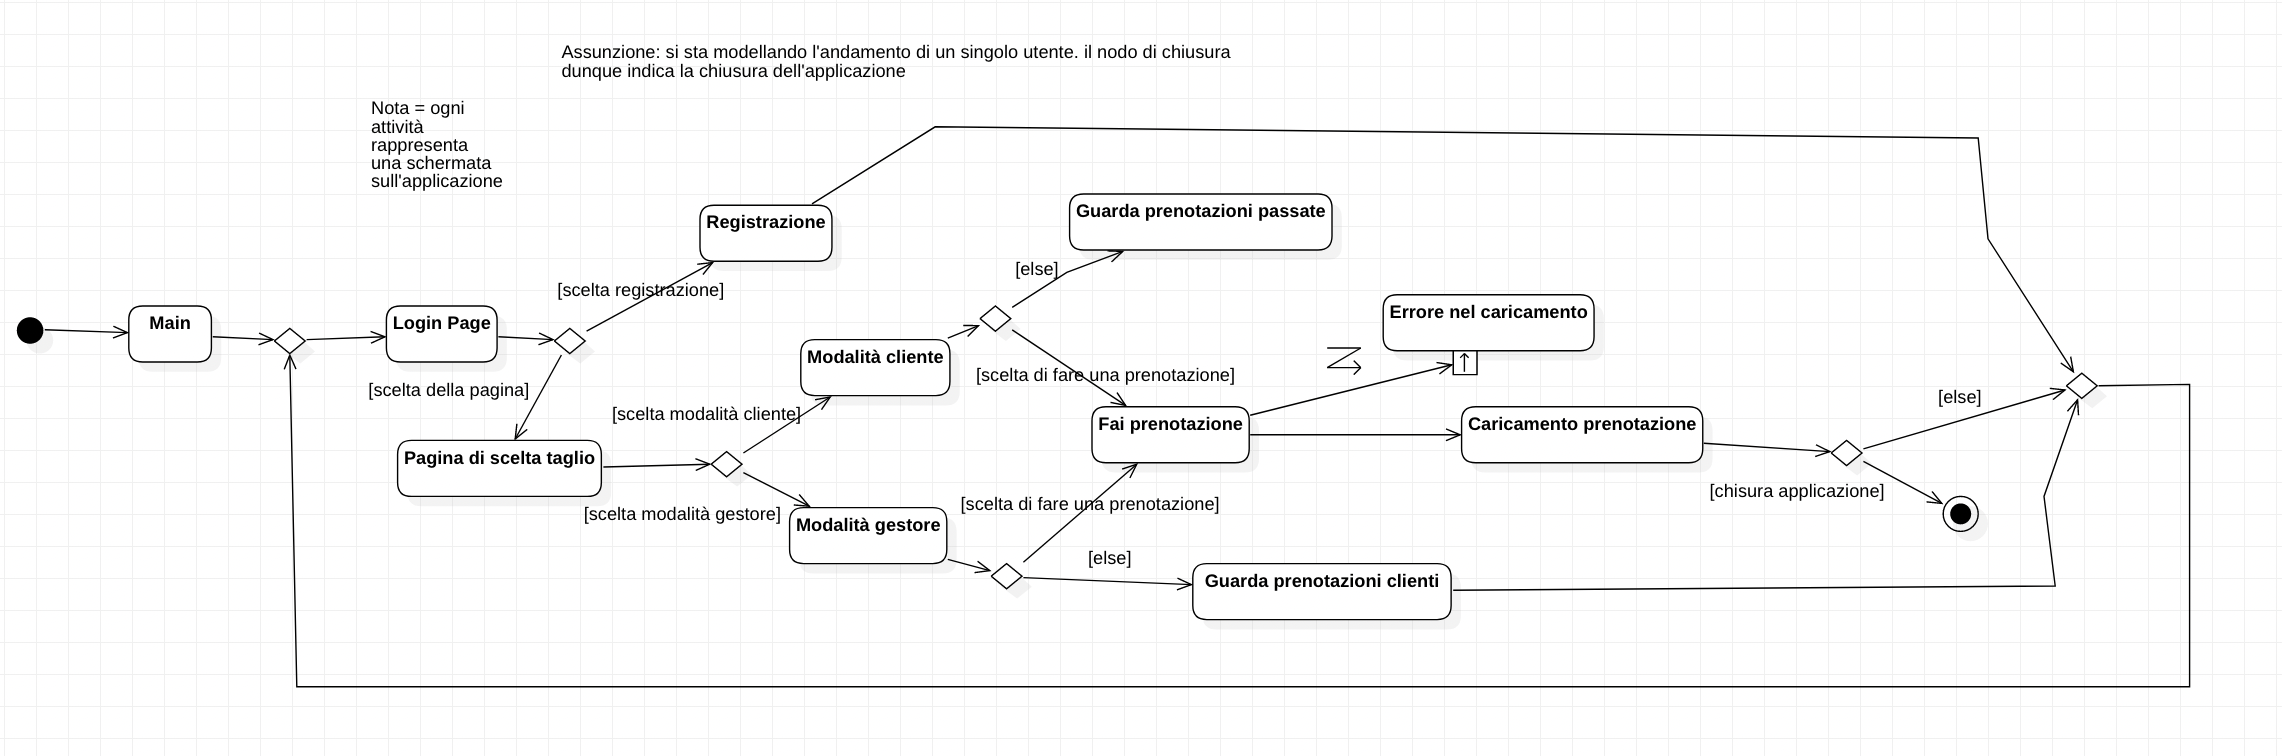
\includegraphics[scale = 0.45]{ImmaginiUML/Activity2.png}
\subsection{funzionamento del programma con una granularità alta}
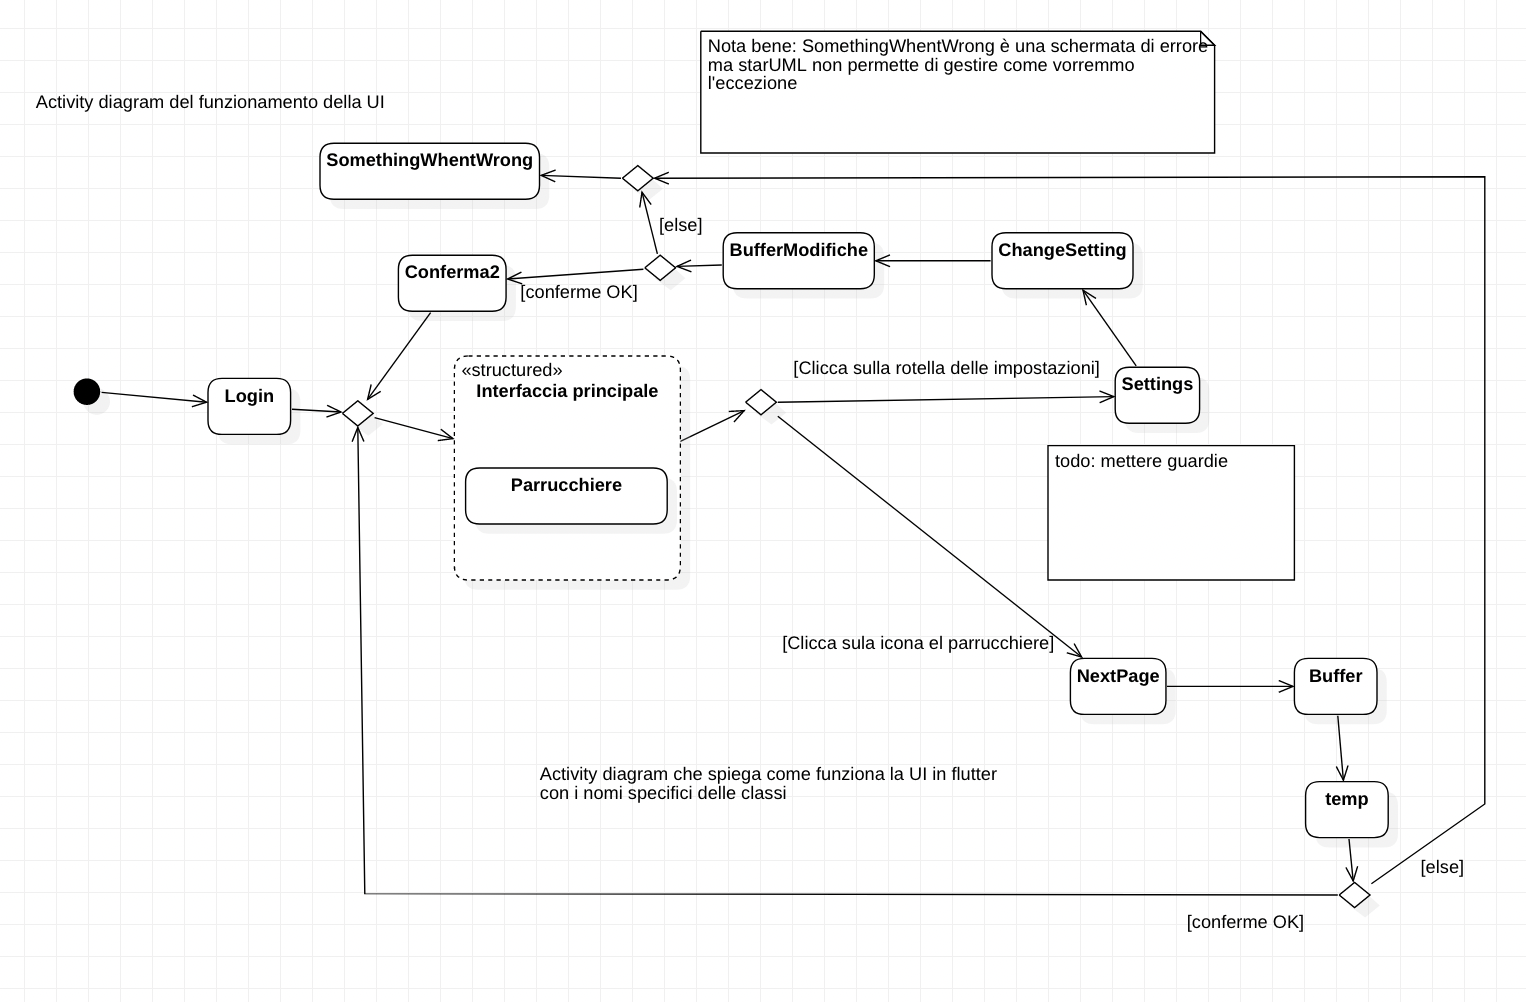
\includegraphics[scale = 0.35]{ImmaginiUML/Activity3.jpg}


\end{document}
